\subsection{Reconstruction des jets}\label{chapter-CMS-section-jets_reco}
La phénoménologie des jets est présentée dans le chapitre~\refChMSSM.
Les partons, \ie\ les quarks et les gluons, ne peuvent pas être directement observés dans le détecteur.
Leur signature expérimentale est un jet, \ie\ un flux collimé de particules stables composé de hadrons, de leptons et de photons.
%\par
Afin de pouvoir étudier le processus initial dont sont issus les partons à l'origine des jets observés, il est nécessaire de reconstruire ces jets en regroupant l'ensemble des particules les constituant.
Des critères d'identification en tant que jet sont imposés à ces regroupements.
Les jets ainsi obtenus sont alors calibrés en énergie selon la procédure détaillée au chapitre~\refChJERC.	
\subsubsection{Regroupement des particules}\label{chapter-CMS-section-jets_reco-subsec-algo}
Le regroupement des particules en jets est réalisé par l'algorithme anti-\kT~\cite{Cacciari_antikT}.
Il s'agit d'un algorithme de recombinaison séquentielle,
dans lequel chaque particule forme initialement un pseudo-jet d'une seule particule~\cite{Cacciari:2011ma}.
\par
La distance $d_{ij}$ entre deux jets $i$ et $j$ est définie par
\begin{equation}
d_{ij} = \min\left(\frac{1}{{\pT}_i^2}, \frac{1}{{\pT}_j^2}\right) \, \frac{\Delta R_{ij}^2}{R^2}
\mend[,]
\end{equation}
où
\begin{equation}
\Delta R_{ij}^2 = (\eta_i-\eta_j)^2 + (\phi_i-\phi_j)^2
\end{equation}
avec $\eta_x$ la pseudo-rapidité,
$\phi_x$ l'angle azimutal et
${\pT}_x$ l'impulsion transverse du jet $x$ et
$R$ un paramètre libre.
De manière itérative et à l'aide de la distance $d_{ij}$, la paire composée des deux jets les plus proches fusionne tant que la distance entre eux est en-deçà d'une valeur seuil.
Les jets fusionnés donnent la liste des jets de l'événement.
\par
Sur la figure~\ref{fig-Jet_PF_Composition_RunII} sont illustrées les compositions des jets reconstruits lors des trois années du Run~II.
Les hadrons sont les composants majoritaires des jets,
avec une contribution de
\num{30} à \SI{60}{\%}
au contenu total
provenant des hadrons chargés
et de
\num{5} à \SI{25}{\%}
des hadrons neutres.
Pour des jets de bas \pT,
la fraction de particules issues de l'empilement peut être de l'ordre de \SI{20}{\%}.
Pour $\pT>\SI{50}{\GeV}$, elles représentent mois de \SI{10}{\%} du contenu des jets.
La proportion de photons augmente avec l'impulsion transverse des jets,
de \SI{25}{\%} à bas \pT\
à
environ \SI{40}{\%} pour $\pT\gtrsim\SI{1}{\TeV}$.
Les électrons et muons représentent moins de \SI{5}{\%} des particules.
L'écart entre données réelles et simulées n'excède généralement pas \SI{2}{\%}.
\begin{figure}[h]
\centering
\subcaptionbox{Année 2016.\label{subfig-Jet_PF_Composition_2016}}[.3\textwidth]
{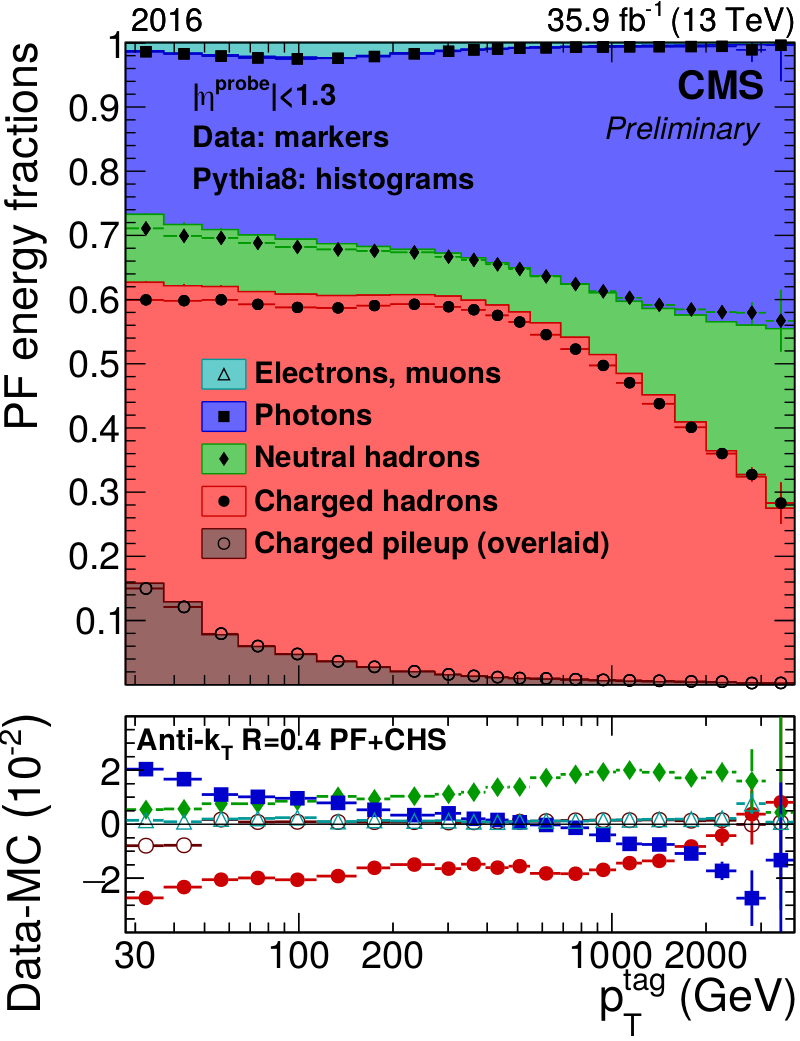
\includegraphics[width=.3\textwidth]{\PhDthesisdir/plots_and_images/from_CMS-DP-2020-019/Jet_PF_Composition_2016.png}}
\hfill
\subcaptionbox{Année 2017.\label{subfig-Jet_PF_Composition_2017}}[.3\textwidth]
{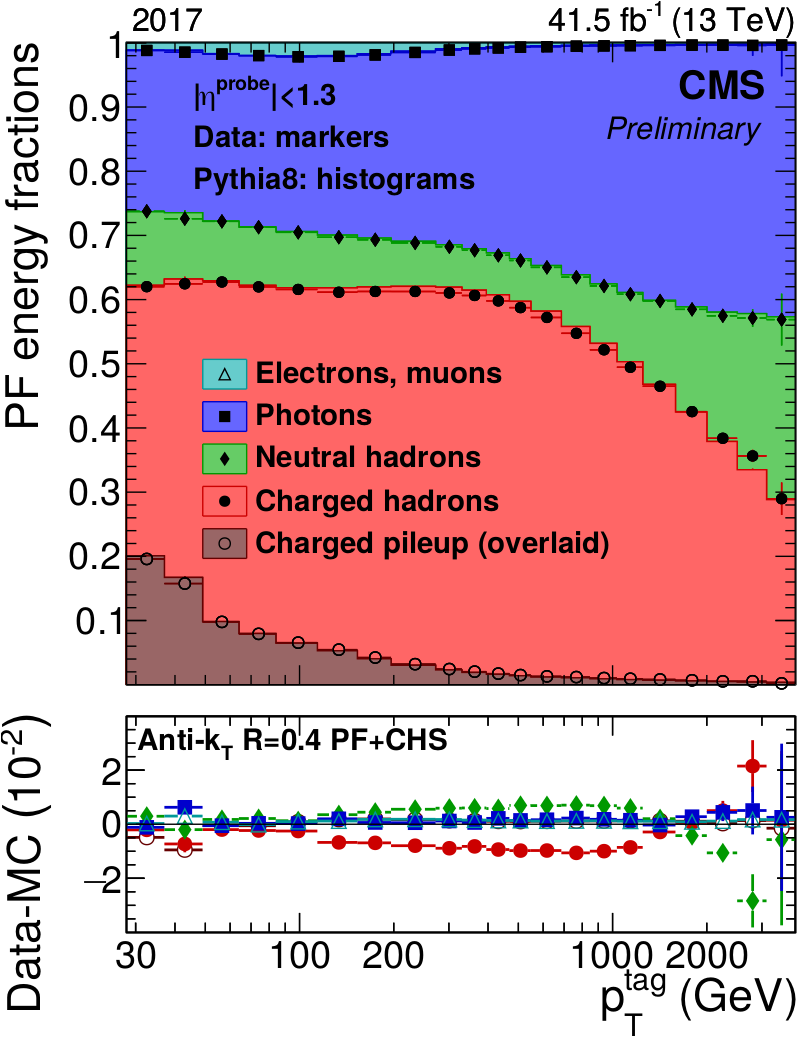
\includegraphics[width=.3\textwidth]{\PhDthesisdir/plots_and_images/from_CMS-DP-2020-019/Jet_PF_Composition_2017.png}}
\hfill
\subcaptionbox{Année 2018.\label{subfig-Jet_PF_Composition_2018}}[.3\textwidth]
{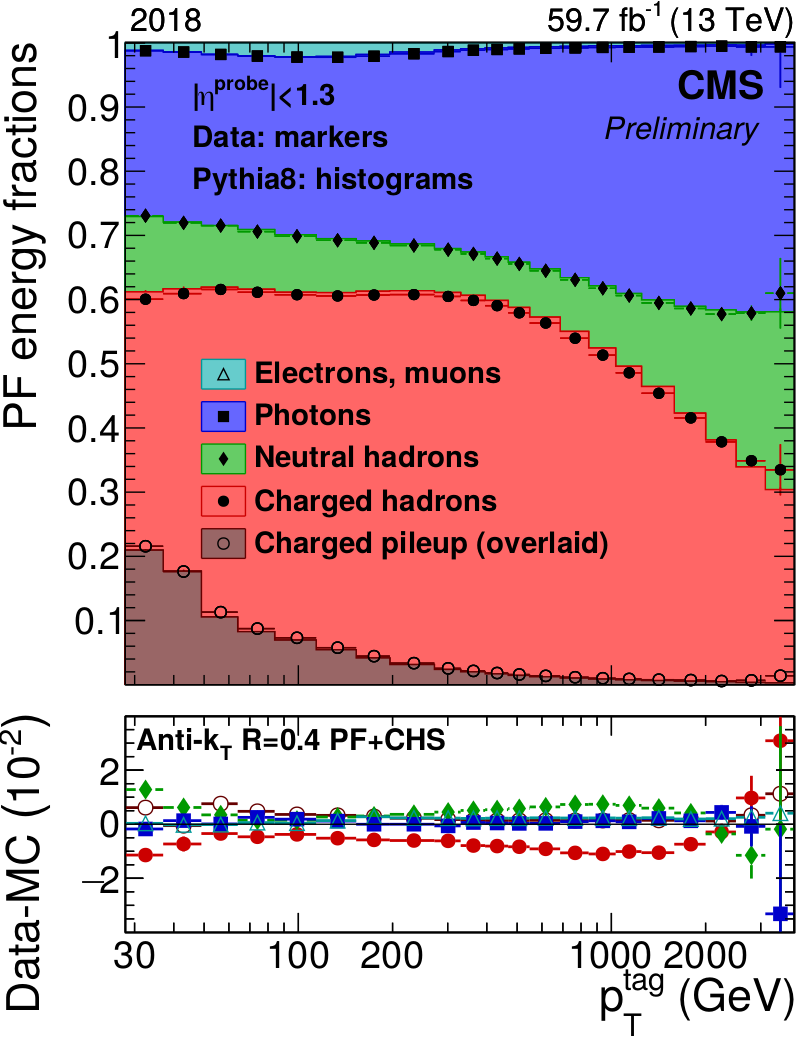
\includegraphics[width=.3\textwidth]{\PhDthesisdir/plots_and_images/from_CMS-DP-2020-019/Jet_PF_Composition_2018.png}}
\caption[Compositions des jets reconstruits lors du Run~II.]{Composition des jets reconstruits à l'aide de l'algorithme anti-\kT\ lors du Run~II~\cite{CMS-DP-2020-019} en fonction de l'impulsion transverse du jet dans les données réelles (Data, histogrammes avec des points) et simulées (MC, histogrammes en couleurs). La partie \emph{Charged pileup (overlaid)} en brun correspond à la fraction du jet retirée par la procédure CHS décrite dans le chapitre~\refChJERC.}
\label{fig-Jet_PF_Composition_RunII}
\end{figure}
\subsubsection{Identification des jets}\label{chapter-CMS-section-jets_reco-subsec-jetID}
Les jets obtenus par regroupement des particules sont en réalité des \og candidats \fg{} jets.
À l'instar des particules individuelles, des critères d'identification leurs sont appliqués afin de rejeter le bruit de fond et de s'assurer de la qualité des jets utilisés dans les analyses.
\par
Ces critères reposent sur les caractéristiques des candidats jets tels que la fraction d'énergie provenant de leurs constituants neutres ou encore le nombre de ces constituants.
Ils dépendent des années de prise de données et de la pseudo-rapidité du jet, \ie\ de la région du détecteur dans laquelle il se trouve.
\par Les critères utilisés pour les années 2016, 2017, 2018, 2017-UL et 2018-UL, listés page~\pageref{tab-chapter-CMS-section-jets_reco-subsec-jetID-2017UL}, permettent d'obtenir une efficacité d'identification des jets supérieure à \SI{99}{\%} dans chacune des régions en $\eta$ du détecteur.
La dénomination \og UL \fg{} signifie \emph{Ultra-Legacy} et correspond à une réinterprétation des données récoltées une fois que la collaboration peut prendre plus de recul sur l'obtention de celles-ci.
La réjection du bruit de fond est supérieure à \SI{98}{\%} pour $\abs{\eta}\leq\num{3.0}$ et supérieure à \SI{36}{\%} pour $\abs{\eta}>\num{3.0}$.
\begin{table}[p]
\centering
\begin{tabularx}{\textwidth}{lcYcY}
\toprule
Propriété du jet à identifier & $\abs{\eta}\leq\num{2.4}$ & $\num{2.4}<\abs{\eta}\leq\num{2.7}$ & $\num{2.7}<\abs{\eta}\leq\num{3.0}$ & $\num{3.0}<\abs{\eta}$ \\
\midrule
Fraction d'énergie\\
\labelitemi\ hadronique neutre & $<\num{0.90}$ & $<\num{0.90}$ & $<\num{0.98}$ & \\
\labelitemi\ électromagnétique neutre & $<\num{0.90}$ & $<\num{0.90}$ & $>\num{0.01}$ & $<\num{0.90}$ \\
\labelitemi\ hadronique chargée & $>\num{0}$ &&&\\
\labelitemi\ électromagnétique chargée & $<\num{0.99}$ &&&\\
\midrule
Nombre de constituants\\
\labelitemi\ neutres & $>\num{1}$ & $>\num{1}$ & $>\num{2}$ & $>\num{10}$ \\
\labelitemi\ chargés & $>\num{0}$ &&&\\
\bottomrule
\end{tabularx}

\caption[Critères d'identification des jets pour l'année 2016.]{Critères d'identification des jets à CMS pour l'analyse des données de 2016.}
\label{tab-chapter-CMS-section-jets_reco-subsec-jetID-2016}
\end{table}
\begin{table}[p]
\centering
\begin{tabularx}{\textwidth}{lcYcY}
\toprule
Propriété du jet à identifier & $\abs{\eta}\leq\num{2.4}$ & $\num{2.4}<\abs{\eta}\leq\num{2.7}$ & $\num{2.7}<\abs{\eta}\leq\num{3.0}$ & $\num{3.0}<\abs{\eta}$ \\
\midrule
Fraction d'énergie\\
\labelitemi\ hadronique neutre & $<\num{0.90}$ & $<\num{0.90}$ &  & $>\num{0.02}$ \\
\labelitemi\ électromagnétique neutre & $<\num{0.90}$ & $<\num{0.90}$ & $<\num{0.99}$ et $>\num{0.02}$ & $<\num{0.90}$ \\
\labelitemi\ hadronique chargée & $>\num{0}$ &&&\\
\labelitemi\ électromagnétique chargée & $<\num{0.8}$ \\
\labelitemi\ muonique & $<\num{0.8}$ & $<\num{0.8}$ \\
\midrule
Nombre de constituants & $>\num{1}$ & $>\num{1}$\\
\labelitemi\ neutres & & & $>\num{2}$ & $>\num{10}$ \\
\labelitemi\ chargés & $>\num{0}$ &&&\\
\bottomrule
\end{tabularx}

\caption[Critères d'identification des jets pour l'année 2017.]{Critères d'identification des jets à CMS pour l'analyse des données de 2017.}
\label{tab-chapter-CMS-section-jets_reco-subsec-jetID-2017}
\end{table}
\begin{table}[p]
\centering
\begin{tabularx}{\textwidth}{lcYcY}
\toprule
Propriété du jet à identifier & $\abs{\eta}\leq\num{2.6}$ & $\num{2.6}<\abs{\eta}\leq\num{2.7}$ & $\num{2.7}<\abs{\eta}\leq\num{3.0}$ & $\num{3.0}<\abs{\eta}\leq\num{5.0}$ \\
\midrule
Fraction d'énergie\\
\labelitemi\ hadronique neutre & $<\num{0.90}$ & $<\num{0.90}$ &  & $>\num{0.2}$ \\
\labelitemi\ électromagnétique neutre & $<\num{0.90}$ & $<\num{0.99}$ & $<\num{0.99}$ et $>\num{0.02}$ & $<\num{0.90}$ \\
\labelitemi\ hadronique chargée & $>\num{0}$ &&&\\
\midrule
Nombre de constituants & $>\num{1}$\\
\labelitemi\ neutres & & & $>\num{2}$ & $>\num{10}$ \\
\labelitemi\ chargés & $>\num{0}$ & $>\num{0}$ &&\\
\bottomrule
\end{tabularx}

\caption[Critères d'identification des jets pour l'année 2018.]{Critères d'identification des jets à CMS pour l'analyse des données de 2018.}
\label{tab-chapter-CMS-section-jets_reco-subsec-jetID-2018}
\end{table}
\begin{table}[p]
\centering
\begin{tabularx}{\textwidth}{lcYcY}
\toprule
Propriété du jet à identifier & $\abs{\eta}\leq\num{2.6}$ & $\num{2.6}<\abs{\eta}\leq\num{2.7}$ & $\num{2.7}<\abs{\eta}\leq\num{3.0}$ & $\num{3.0}<\abs{\eta}\leq\num{5.0}$ \\
\midrule
Fraction d'énergie\\
\labelitemi\ hadronique neutre & $<\num{0.90}$ & $<\num{0.90}$ &  & $>\num{0.2}$ \\
\labelitemi\ électromagnétique neutre & $<\num{0.90}$ & $<\num{0.99}$ & $<\num{0.99}$ et $>\num{0.01}$ & $<\num{0.90}$ \\
\labelitemi\ hadronique chargée & $>\num{0}$ &&&\\
\labelitemi\ électromagnétique chargée & $<\num{0.8}$ & $<\num{0.8}$ \\
\labelitemi\ muonique & $<\num{0.8}$ & $<\num{0.8}$ \\
\midrule
Nombre de constituants & $>\num{1}$\\
\labelitemi\ neutres & & & $>\num{1}$ & $>\num{10}$ \\
\labelitemi\ chargés & $>\num{0}$ & $>\num{0}$ &&\\
\bottomrule
\end{tabularx}

\caption[Critères d'identification des jets pour les années 2017-UL et 2018-UL.]{Critères d'identification des jets à CMS pour l'analyse des données de 2017-UL et 2018-UL.}
\label{tab-chapter-CMS-section-jets_reco-subsec-jetID-2017UL}
\end{table}
\subsubsection{Saveur des jets}\label{chapter-CMS-section-jets_reco-subsec-flavor}
%Pour étudier la physique du processus initial, la connaissance du parton à l'origine d'un jet ainsi identifié dans le détecteur est une information de choix.
Il est impossible de connaître avec certitude le parton à l'origine d'un jet,
mais ce dernier possède des propriétés caractéristiques dépendantes du parton, comme exposé dans le chapitre~\refChMSSM.
%Il est impossible de connaître avec certitude cette particule, mais sa nature influe directement sur certaines propriétés des jets, comme exposé dans le chapitre~\refChMSSM.
\par
%Comme exposé dans le chapitre~\refChMSSM,
%les jets présentent des propriétés caractéristiques, selon le parton à leur origine qu'il s'agisse de jets légers (quarks~\quarkd, \quarku\ ou~\quarks), de jets lourds (quarks~\quarkc\ ou~\quarkb) ou de jets issus d'un gluon.
En utilisant ces propriétés, des algorithmes d'identification de la saveur des jets ont été mis au point par la collaboration CMS~\cite{jet_btag_CSV_RunI}.
Les avancées récentes dans le domaine du \emph{Deep Learning}, appliquées à l'identification des jets~\cite{jet_flavor_deep_nn}, ont permis l'amélioration de ces algorithmes.
\DeepCSV~\cite{Sirunyan_heavy_flavor_jets_2018} en est un exemple.
\par Les variables utilisées dans cet algorithme, décrites dans la référence~\cite{Sirunyan_heavy_flavor_jets_2018},
sont traitées par un réseau de neurones profond composé de quatre couches cachées de 100 nœuds connectés les uns aux autres.
Le principe des réseaux de neurones est abordé plus en détail dans le chapitre~\refChML.
Ce réseau a été entraîné à l'aide des librairies
\KERAS~\cite{keras}
et
\TENSORFLOW~\cite{tensorflow}
sur un ensemble d'événements simulés \ttbar, présentant de nombreux jets de quarks~\quarkb, et multijet.
\par Les performances ainsi obtenues pour l'algorithme \DeepCSV\ sont comparées à d'autres algorithmes d'identification de la saveur des jets sur la figure~\ref{fig-chapter-CMS-section-jets_reco-subsec-flavor-bc_tag_roc_curves}.
Les algorithmes \textsc{cMVAv2} et \DeepCSV\ présentent les meilleures performances en termes d'identification des jets de quark~\quarkb\ (\quarkb-\emph{tagging}).
Pour le traitement des jets de quark~\quarkc, l'algorithme \DeepCSV\ propose les meilleures performances.
Dans les analyses présentées dans les chapitres~\refChJERC\ et~\refChHTT, c'est cet algorithme qui est utilisé afin d'identifier les jets issus de quarks~\quarkc\ ou~\quarkb.
\begin{figure}[h]
\centering

\subcaptionbox{Probabilité de mauvaise identification en tant que jet de quark~\quarkb\ de jets de gluon ou quarks légers (traits pleins) ou de jets de quark~\quarkc\ (pointillés) en fonction de l'efficacité d'identification des jets de quark~\quarkb.\label{subfig-chapter-CMS-section-jets_reco-subsec-flavor-b_or_mis}}[.75\textwidth]
{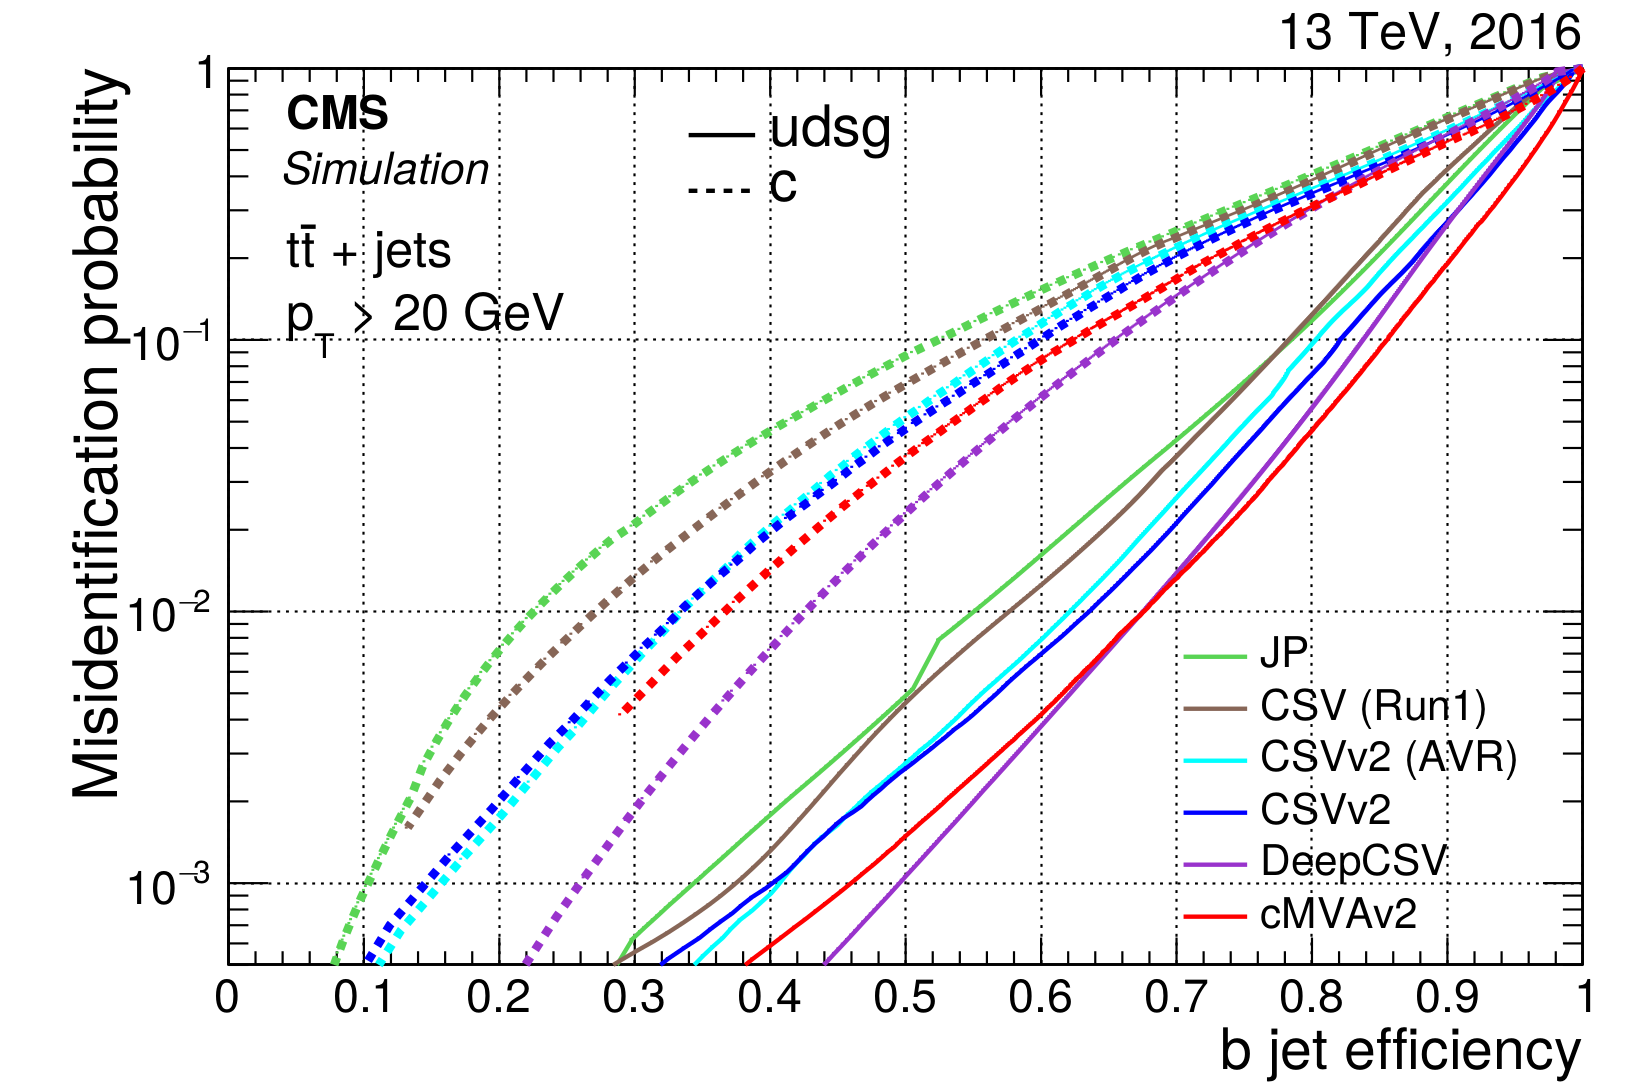
\includegraphics[width=.45\textwidth]{\PhDthesisdir/plots_and_images/from_Sirunyan_heavy_flavor_jets_2018/b_or_mis.png}}

\vspace{\baselineskip}

\subcaptionbox{Probabilité de mauvaise identification en tant que jet de quark~\quarkc\ de jets de gluon ou quarks légers en fonction de l'efficacité d'identification des jets de quark~\quarkc.\label{subfig-chapter-CMS-section-jets_reco-subsec-flavor-c_or_mis}}[.45\textwidth]
{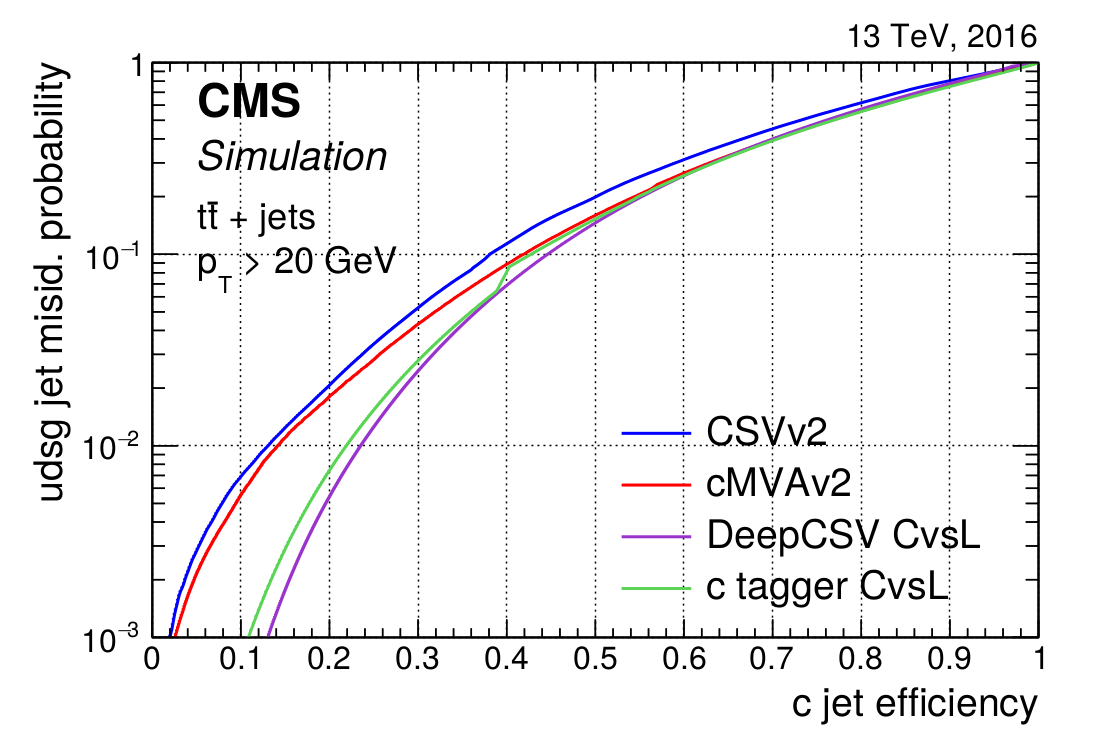
\includegraphics[width=.45\textwidth]{\PhDthesisdir/plots_and_images/from_Sirunyan_heavy_flavor_jets_2018/c_or_mis.png}}
\hfill
\subcaptionbox{Probabilité de mauvaise identification en tant que jet de quark~\quarkb\ de jets de quark~\quarkc\ en fonction de l'efficacité d'identification des jets de quark~\quarkc.\label{subfig-chapter-CMS-section-jets_reco-subsec-flavor-c_or_b}}[.45\textwidth]
{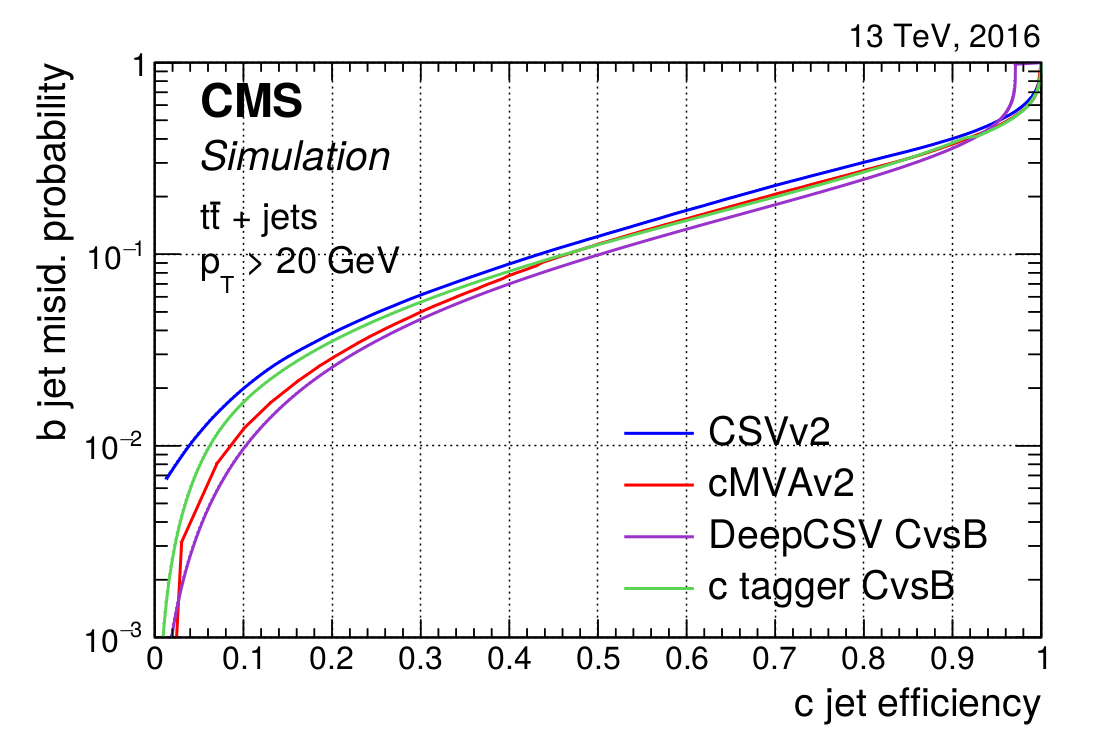
\includegraphics[width=.45\textwidth]{\PhDthesisdir/plots_and_images/from_Sirunyan_heavy_flavor_jets_2018/c_or_b.png}}

\caption[Performances des algorithmes d'identification de la saveur des jets.]{Comparaison des performances des algorithmes d'identification de la saveur des jets~\cite{Sirunyan_heavy_flavor_jets_2018}.}
\label{fig-chapter-CMS-section-jets_reco-subsec-flavor-bc_tag_roc_curves}
\end{figure}
%\par La discrimination entre jet léger et jet initié par un gluon peut être réalisée à l'aide d'une fonction de vraisemblance~\cite{CMS-PAS-JME-13-002} donnant un score entre 0 et 1 pour chaque jet, correspondant à la probabilité que ce jet soit issu d'un quark. La densité de probabilité de cette fonction, selon qu'il s'agisse de jets initiés par des gluons ou des quarks, est représentée sur la figure~\ref{fig-chapter-CMS-section-jets_reco-subsec-flavor-qgl_likelihood}.
%\begin{figure}[h]
%\centering
%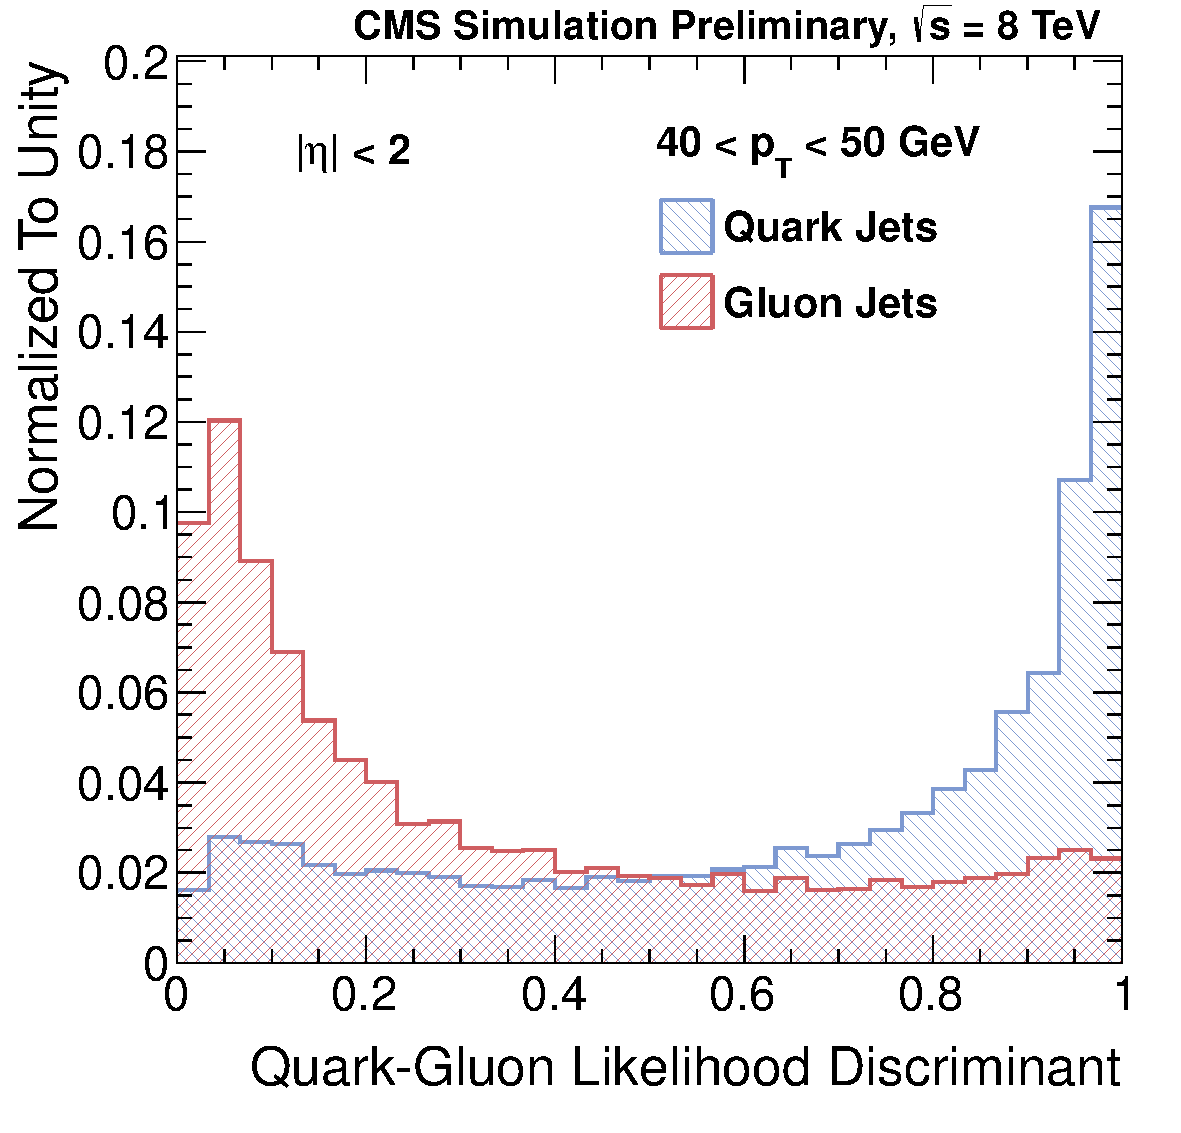
\includegraphics[width=.45\textwidth]{\PhDthesisdir/plots_and_images/from_CMS-PAS-JME-13-002/qgl.pdf}
%\caption[Performances de la discrimation quark-gluon pour la saveur des jets.]{Densité de probabilité de la fonction de vraisemblance utilisée pour discriminer les jets issus de gluons de ceux issus de quarks~\cite{CMS-PAS-JME-13-002}. En rouge, pour les jets issus de gluons. En bleu, pour des jets issus de quarks.}
%\label{fig-chapter-CMS-section-jets_reco-subsec-flavor-qgl_likelihood}
%\end{figure}